% !TEX encoding = UTF-8 Unicode
%!TEX root = thesis.tex
% !TEX spellcheck = en-US
%%=========================================
\chapter{Results}

The results will be introduced in the same order as the experiments were conducted. First, the results of matching of one of the EDX datasets with the SPED dataset will be presented. This is followed the position matching of the various EDX datasets with the overview images. Lastly, the calculated $\zeta$-factors and the quantification of the samples using the $\zeta$-factor method and the Cliff-Lorimer technique are displayed.

\section{Dataset matching}

\cref{fig:edx-in-sped} shows the results of matching the largest EDX dataset with the SPED dataset. As explained in \cref{sec:method/dataset matching}, these images have been processed to be made more similar. \cref{fig:edx-in-sped} shows the processed EDX image and \cref{fig:edx-in-sped-rectangle} shows the processed SPED image with a rectangle indicating where the EDX image fit best. 

\begin{figure}
\begin{subfigure}{.5\textwidth}
	\centering
	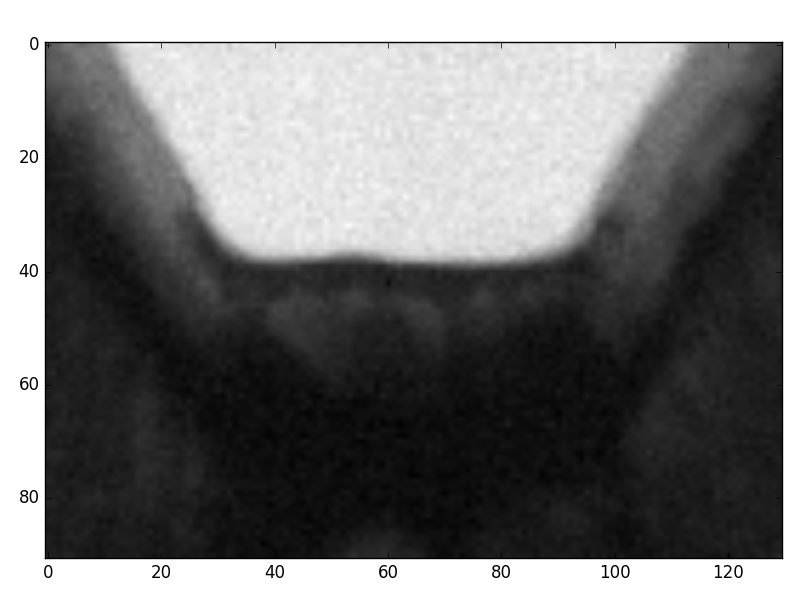
\includegraphics[width=\linewidth]{fig/se_image_in_sped_with_rectangle.png}
	\caption{++++++}
	\label{fig:edx-in-sped-edx}
\end{subfigure}%
\begin{subfigure}{.5\textwidth}
	\centering
	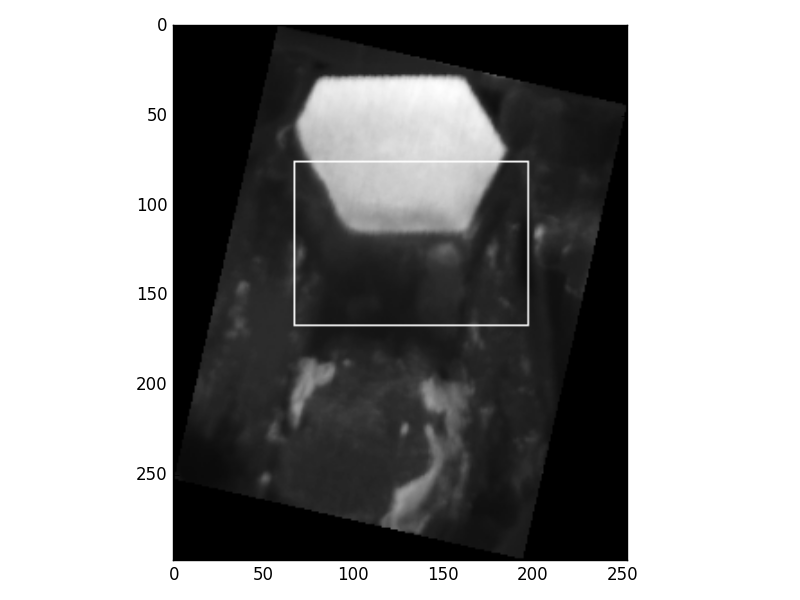
\includegraphics[width=\linewidth]{fig/sped-with-rectangle.png}
	\caption{++++++}
	\label{fig:edx-in-sped-rectangle}
\end{subfigure}
\caption{plots of....}
\label{fig:edx-in-sped}
\end{figure}

As the correct result is unknown, it is difficult to quantify the error in the fit. An attempt was made by looking at the difference between the matching value for the best position, shown in \cref{fig:edx-in-sped-rectangle}, and the higher values. The matching values are defined in \cref{eq:matching value}. \cref{fig:edx-sped-rectangle-match-graph} shows the relative error of the 100 best matching values with respect to the best match. 

\begin{figure}
	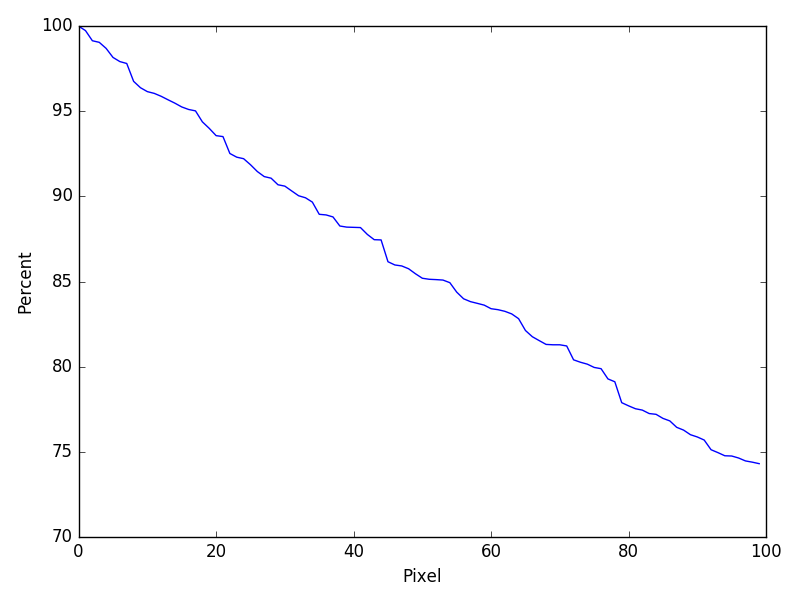
\includegraphics[width=0.7\linewidth]{fig/edx-sped-rectangle-match-graph.png}
	\caption{++++++}
	\label{fig:edx-sped-rectangle-match-graph}
\end{figure}

The results from locating the EDX datasets in the HAADF overview images are displayed in \cref{fig:nonheated-images-in-overview, fig:heated-images-in-overview} for the non-treated and the heat-treated samples, respectively. In the non-treated sample, the two datasets B and D were not correctly located in the overview image. The calculated location of dataset B was completely off, while the position of D was just slightly offset. The actual positions of these datasets were estimated by eye and marked in \cref{fig:nonheated-images-in-overview} as blue dotted rectangles. The rest of the datasets were located correctly, and their positions are shown as red rectangles. For the heat-treated sample, all the datasets that were included in the overview image were correctly located. However, the areas covered by two the datasets A and B were found to not be included in the overview image.

\begin{figure}
	\begin{subfigure}{.5\textwidth}
		\centering
		\includegraphics[width=\linewidth]{"fig/nonheated-images-in-overview (correct)3"}
		\caption{}
		\label{fig:nonheated-images-in-overview}
	\end{subfigure}%
	\begin{subfigure}{.5\textwidth}
		\centering
		\includegraphics[width=\linewidth]{"fig/nonheated-matching-values"}
		\caption{}
		\label{fig:nonheated-matching-values}
	\end{subfigure}
\end{figure}

\begin{figure}
	\begin{subfigure}{.5\textwidth}
		\centering
		\includegraphics[width=\linewidth]{"fig/heated-images-in-overview-ink2"}
		\caption{}
		\label{fig:nonheated-images-in-overview}
	\end{subfigure}%
	\begin{subfigure}{.5\textwidth}
		\centering
		\includegraphics[width=\linewidth]{"fig/heated-matching-values"}
		\caption{}
		\label{fig:nonheated-matching-values}
	\end{subfigure}
\end{figure}

The accuracy of the matching for the different datasets are shown in \cref{fig:nonheated-matching-values} for the non-heated sample, and in \cref{fig:heated-matching-values} for the heated values. The horizontal axis shows the different datasets while the vertical axis is the matching value in percent, where $\SI{100}{\percent}$ is defined to be the matching value of the dataset covering the biggest area in each respective sample. The matching of this dataset is assumed to be the most trustworthy due to there being fewer potential locations that resemble the actual location, as there are several distinct features. For the smaller datasets, or more accurately, the datasets with smaller survey images, there might be several different locations in the overview image that all give a fairly good match.


In both figures, the red star is the value of the dataset used as reference, the red circles are the correctly matched datasets while the blue squares are the datasets that resulted in a wrong location. The non-heated sample (\cref{fig:nonheated-matching-values}) shows high values for all the correctly located datasets, and significantly lower values for the wrongly located ones. In addition, it must be noted that the exact location of dataset F was impossible to verify visually due to the survey image not being large enough to distinguish specific features. In the heated sample (\cref{fig:heated-matching-values}), all the red correctly located datasets have high values while the datasets that were not present in the reference image have distinguishably lower values.

\section{Determination of $\zeta$-values}

The calculated $\zeta$-values for all the elements present in the sample are presented in \cref{tab:non-heated zeta-values}, along with which dataset was used to calculate them. All datasets are from the unheated sample except for C*, which is from the heated one.

\begin{table}
	\caption{...}
	\begin{center}
	\begin{tabular}{ccc}

	Element & Dataset & $\zeta$\\ 
	\midrule
	\hline
	Ga & C* & 582\\
	Ga & A  & 608\\
	As & C* & 689\\
	As & A  & 706\\
	Ge & B  & 732\\
	Ge & D  & 741\\
	Ge & A  & 748\\
	Pd & E  & 1248\\
	Pd & A  & 1284\\
	Pd & B  & 1318\\
%	Au & B  & 3450\\ 
%	Au & C  & 3473\\
	Au & B & 2397\\
	Au & C & 2387\\
	\hline
	\end{tabular} 
	\end{center}
	\label{tab:non-heated zeta-values}
\end{table}

These values have been 


\section{Quantification}

The compositions of the unheated and the heated samples have been quantified using the Cliff-Lorimer ratio method and the $\zeta$-factor method with and without absorption correction. The composition of the unheated sample is known, and can therefore used as a reference for the accuracy of the quantization of the heated sample, whose composition is largely unknown.

\begin{figure}
	\begin{subfigure}{.5\textwidth}
		\centering
		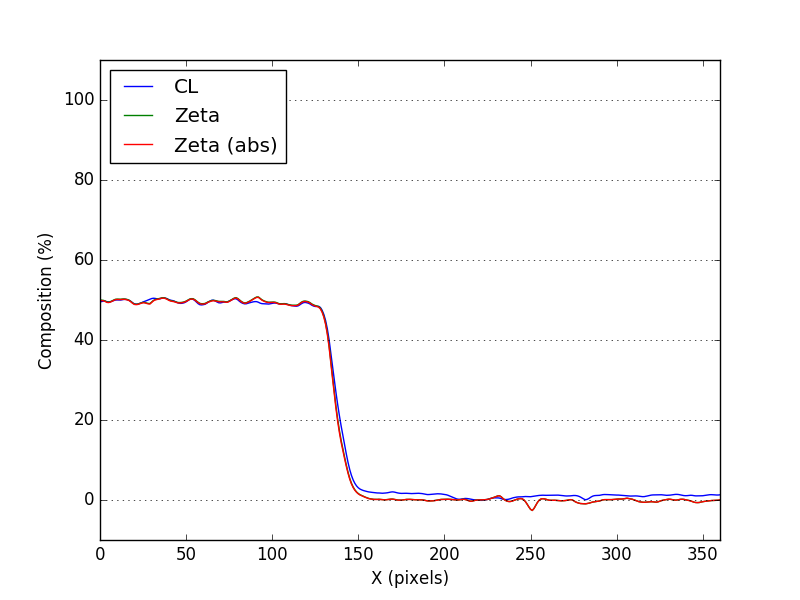
\includegraphics[width=\linewidth]{fig/q/1_ga2}
		\caption{++++++}
		\label{fig:zeta_area1_ga}
	\end{subfigure}%
	\begin{subfigure}{.5\textwidth}
		\centering
		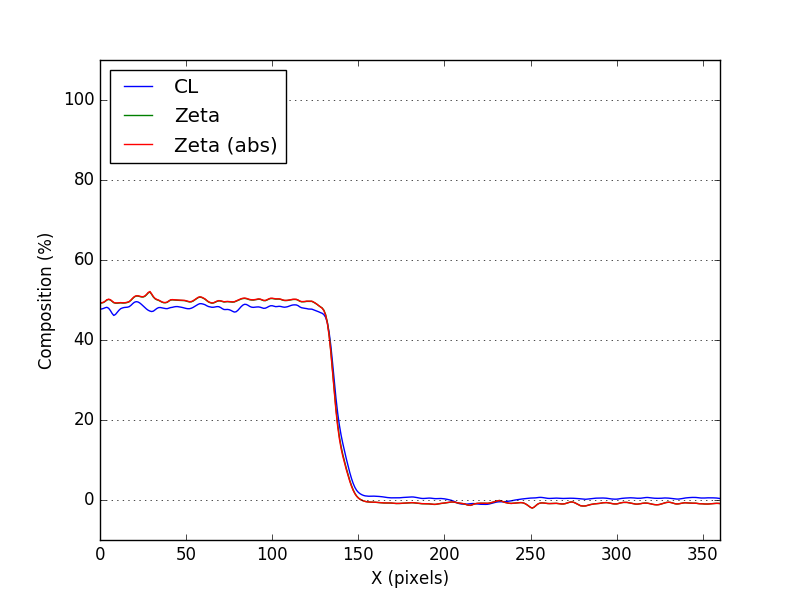
\includegraphics[width=\linewidth]{fig/q/1_as2}
		\caption{++++++}
		\label{fig:zeta_area1_as}
	\end{subfigure}
		\begin{subfigure}{.5\textwidth}
			\centering
			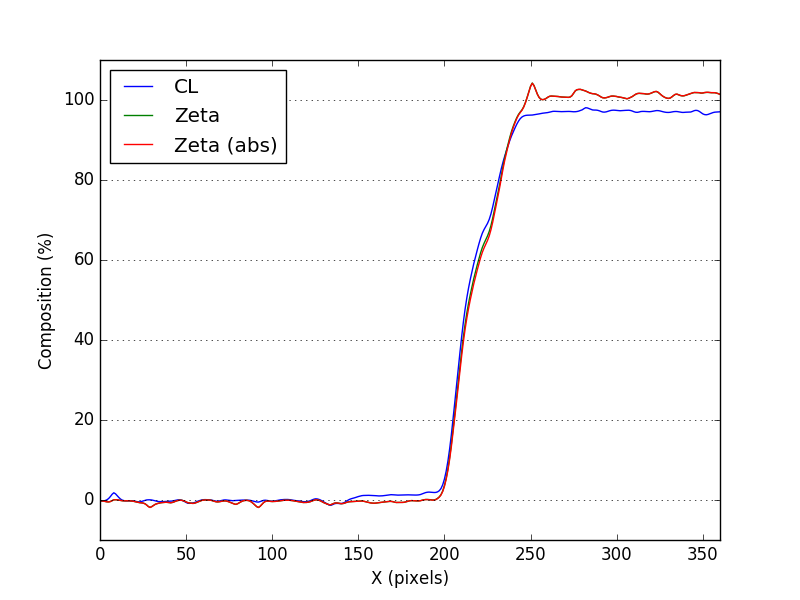
\includegraphics[width=\linewidth]{fig/q/1_ge2}
			\caption{++++++}
			\label{fig:zeta_area1_ge}
		\end{subfigure}%
		\begin{subfigure}{.5\textwidth}
			\centering
			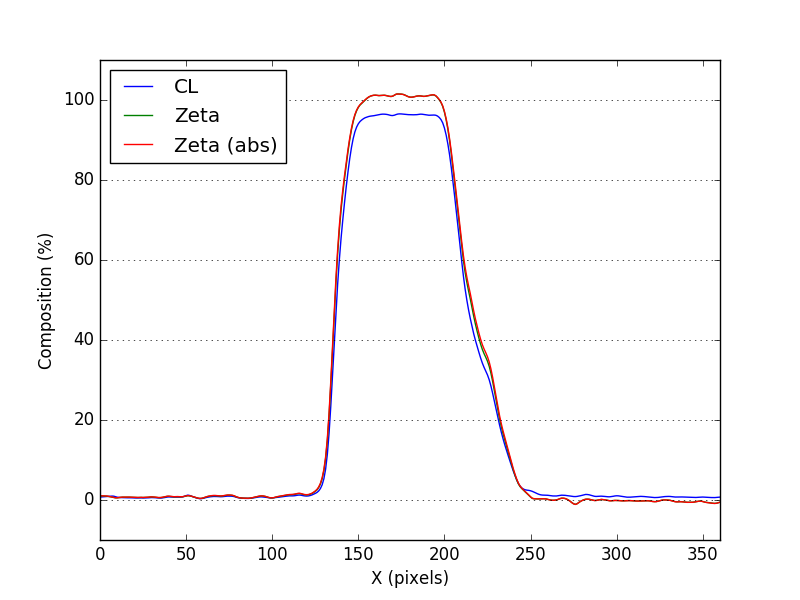
\includegraphics[width=\linewidth]{fig/q/1_pd2}
			\caption{++++++}
			\label{fig:zeta_area1_pd}
	\end{subfigure}
		\begin{subfigure}{.5\textwidth}
			\centering
			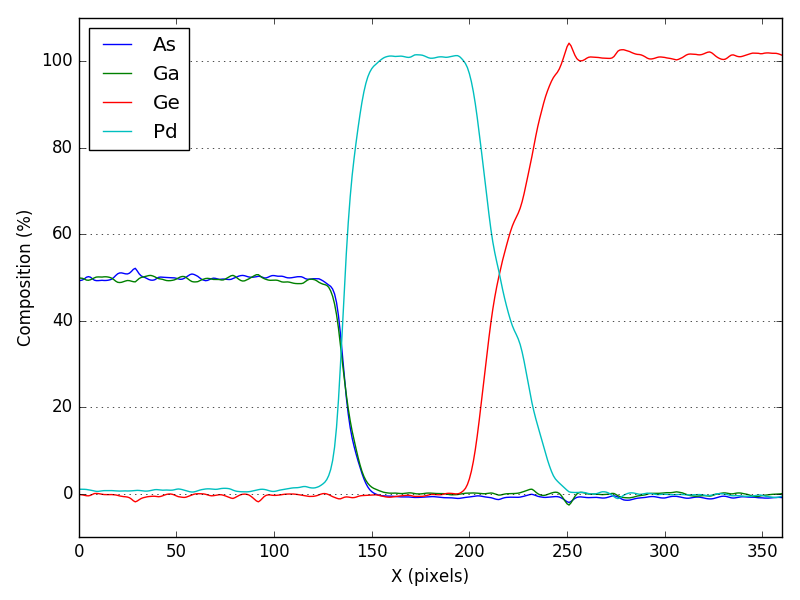
\includegraphics[width=\linewidth]{fig/q/1_all_abscorr2}
			\caption{++++++}
			\label{fig:zeta_area1_all}
	\end{subfigure}%
	\begin{subfigure}{.5\textwidth}
		\centering
		\newlength\imageheight
%		\settoheight\imageheight{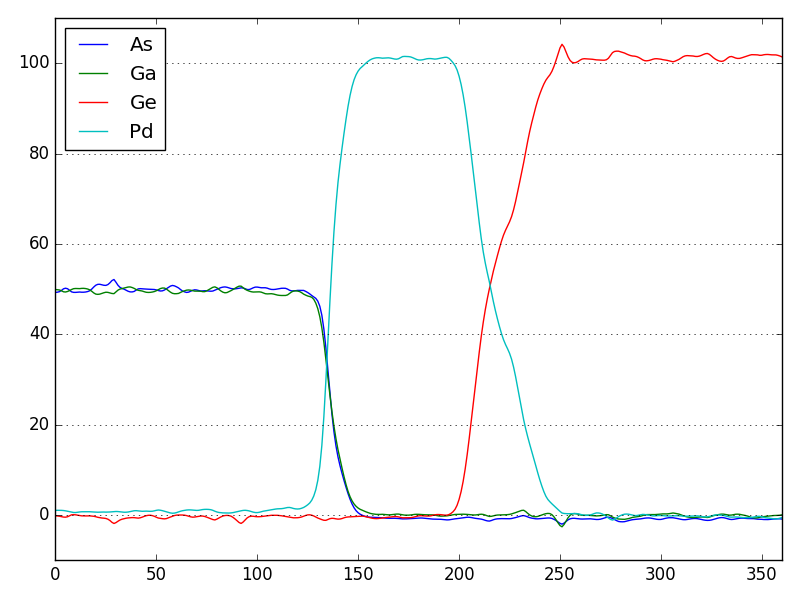
\includegraphics{fig/q/1_all_abscorr}}
%		\newlength\imagewidth
%		\settowidth\imagewidth{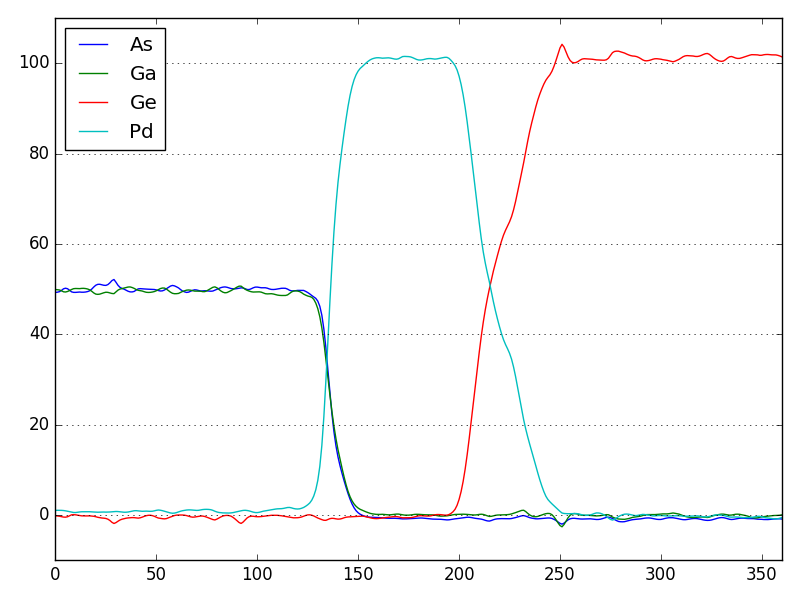
\includegraphics{fig/q/1_all_abscorr}}
		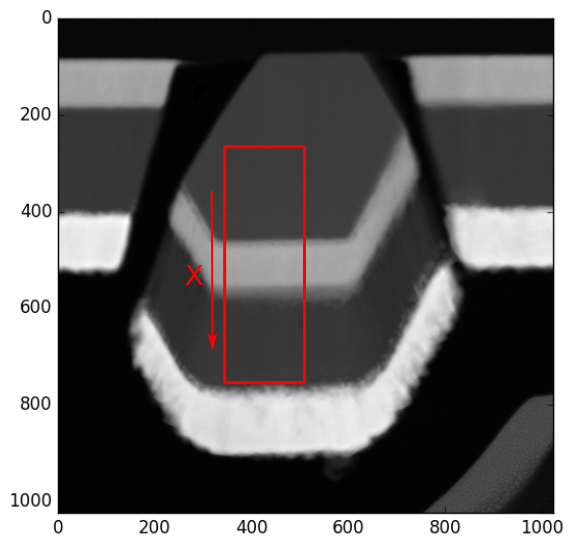
\includegraphics[width=.68\linewidth]{fig/q/1_overview3}
		\caption{++++++}
		\label{fig:zeta_area1_overview}
	\end{subfigure}
	\caption{plots of....}
	\label{fig:zeta_area1}
\end{figure}

\begin{figure}
	\begin{subfigure}{.5\textwidth}
		\centering
		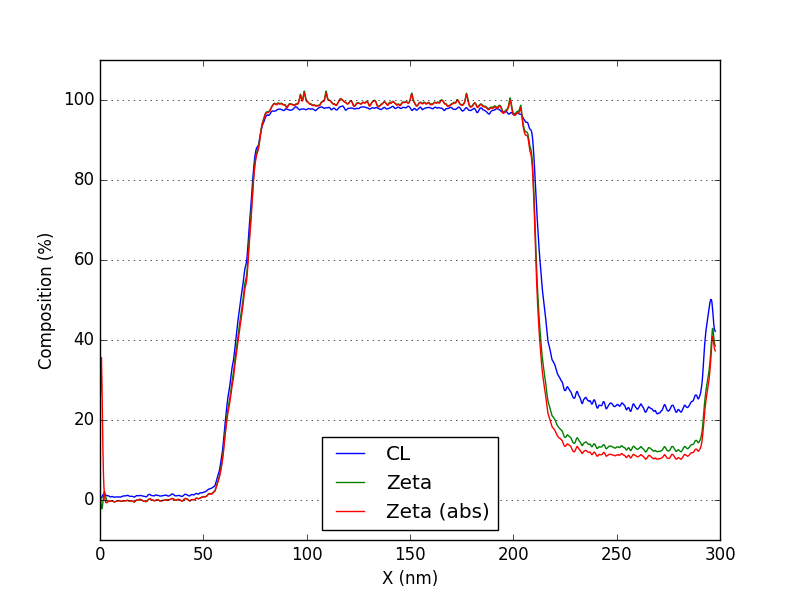
\includegraphics[width=\linewidth]{fig/q/2_ge}
		\caption{++++++}
		\label{fig:zeta_area1_ga}
	\end{subfigure}%
	\begin{subfigure}{.5\textwidth}
		\centering
		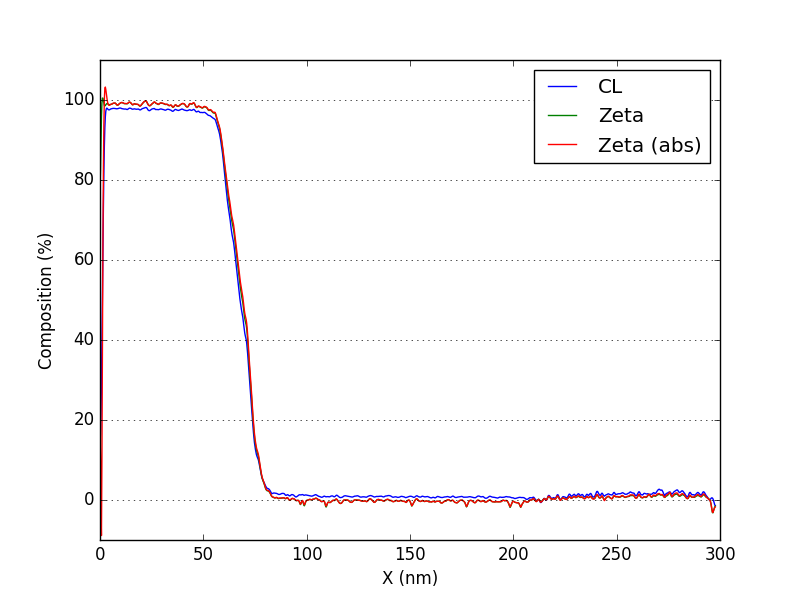
\includegraphics[width=\linewidth]{fig/q/2_pd}
		\caption{++++++}
		\label{fig:zeta_area1_as}
	\end{subfigure}
	\begin{subfigure}{.5\textwidth}
		\centering
		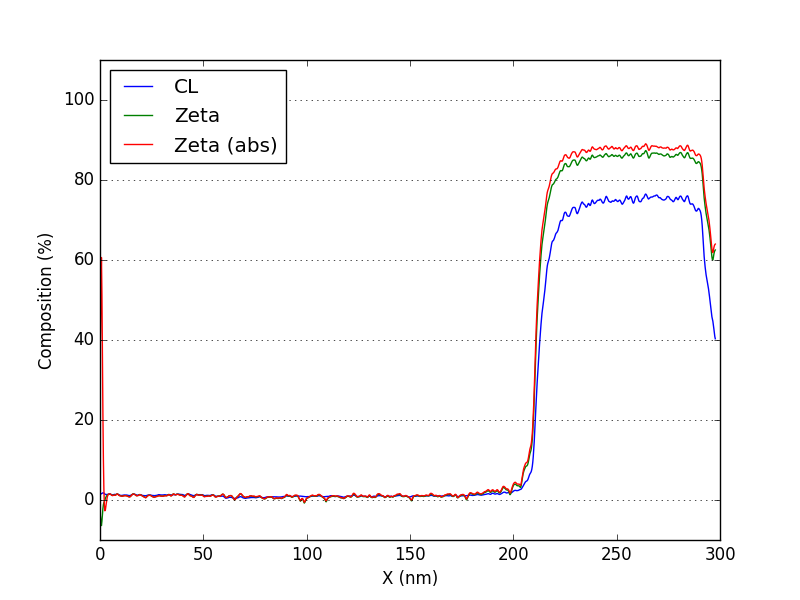
\includegraphics[width=\linewidth]{fig/q/2_au}
		\caption{++++++}
		\label{fig:zeta_area1_ge}
	\end{subfigure}%
	\begin{subfigure}{.5\textwidth}
		\centering
		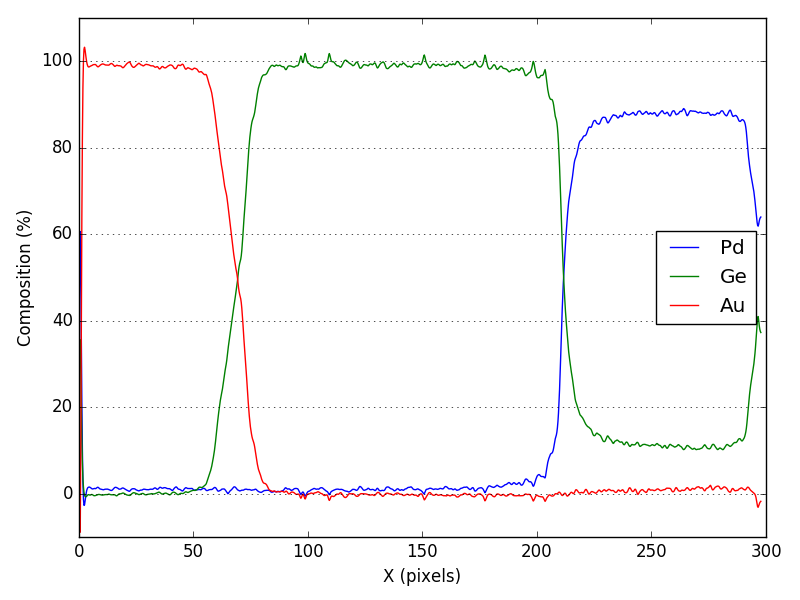
\includegraphics[width=\linewidth]{fig/q/2_all_abscorr}
		\caption{++++++}
		\label{fig:zeta_area1_all}
	\end{subfigure}
		\centering
	\begin{subfigure}{.5\textwidth}
%		\newlength\imageheight
		%		\settoheight\imageheight{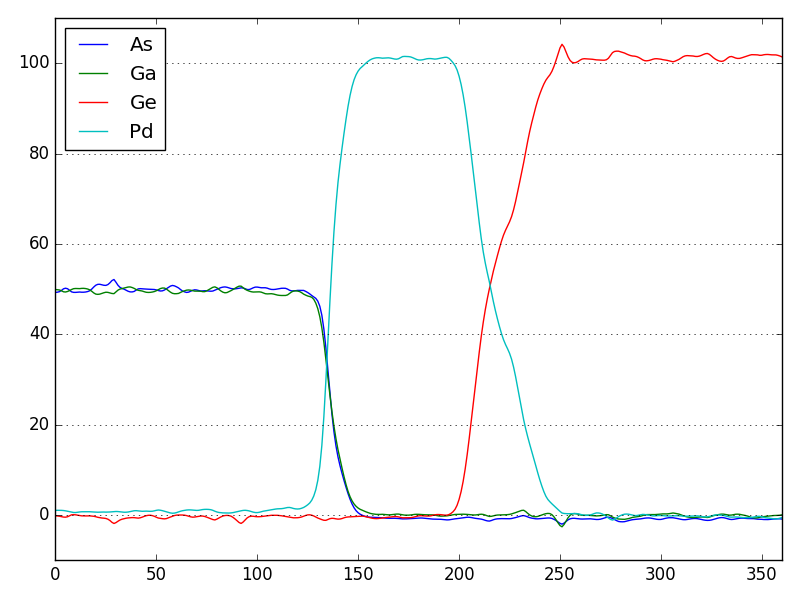
\includegraphics{fig/q/1_all_abscorr}}
		%		\newlength\imagewidth
		%		\settowidth\imagewidth{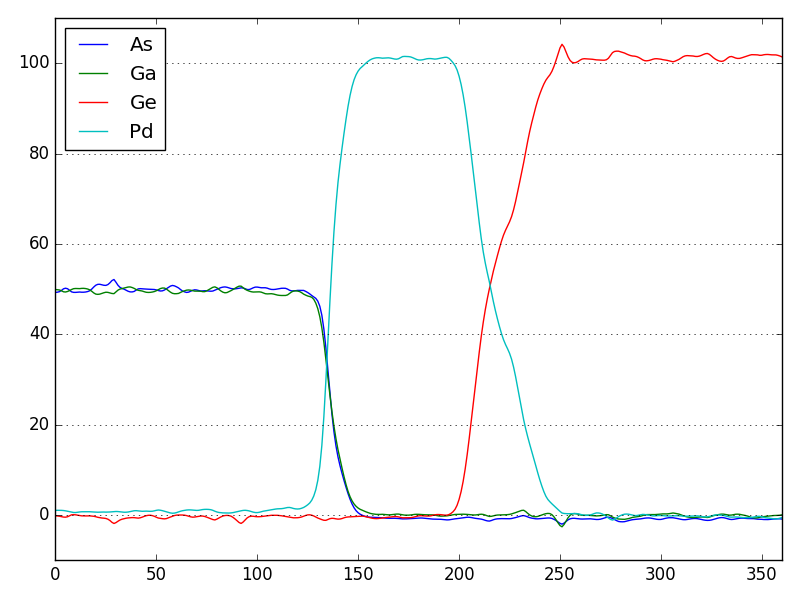
\includegraphics{fig/q/1_all_abscorr}}
		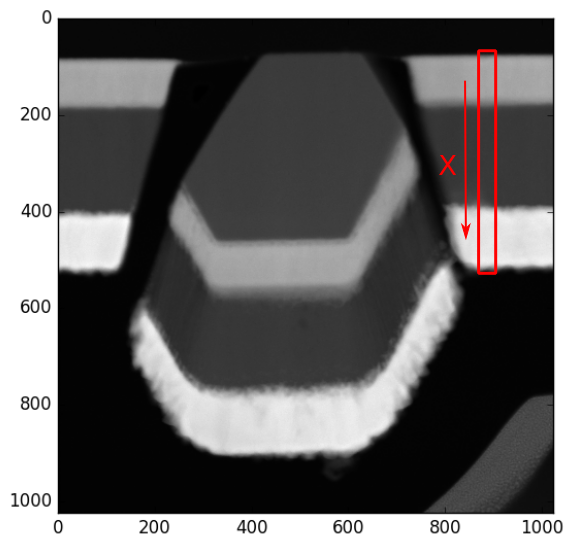
\includegraphics[width=.68\linewidth]{fig/q/2_overview}
		\caption{++++++}
		\label{fig:zeta_area2_overview}
	\end{subfigure}
	\caption{plots of....}
	\label{fig:zeta_area2}
\end{figure}